\documentclass[10pt,a4paper, ngerman]{beamer}

\usepackage[ngerman]{babel}
\usepackage[T1]{fontenc}
\usepackage[utf8]{inputenc}
\usepackage{varioref}
\usepackage{hyperref}
\usepackage{cleveref}
\usepackage{amsmath}
\usepackage{amsfonts}
\usepackage{amssymb}
\usepackage{makeidx}
\usepackage{graphicx}
\usepackage{csquotes}
\usepackage{listings}
\usepackage{color}
\usepackage{xcolor}
\usepackage[most]{tcolorbox}
\usepackage{amssymb}
\usepackage{lmodern}
\usepackage{verbatim}

% Umlaute und ß in Listings
\lstset{basicstyle=\ttfamily}
\lstset{literate=%
  {Ö}{{\"O}}1
  {Ä}{{\"A}}1
  {Ü}{{\"U}}1
  {ß}{{\ss}}1
  {ü}{{\"u}}1
  {ä}{{\"a}}1
  {ö}{{\"o}}1
}

% Farben für Listings
\definecolor{codegreen}{rgb}{0,0.6,0}
\definecolor{codegray}{rgb}{0.5,0.5,0.5}
\definecolor{codepurple}{rgb}{0.58,0,0.82}
\definecolor{backcolour}{rgb}{0.95,0.95,0.92}
 
\lstdefinestyle{mystyle}{
    backgroundcolor=\color{backcolour},   
    commentstyle=\color{codegreen},
    keywordstyle=\color{magenta},
    numberstyle=\tiny\color{codegray},
    stringstyle=\color{codepurple},
    basicstyle=\footnotesize,
    breakatwhitespace=false,         
    breaklines=true,                 
    captionpos=t,                    
    keepspaces=true,                 
    numbers=left,                    
    numbersep=5pt,                  
    showspaces=false,                
    showstringspaces=false,
    showtabs=false,                  
    tabsize=2,
	language=[LaTeX]{TeX}
}

\lstset{style=mystyle}

\definecolor{hbbkBlueish}{HTML}{5e7b87}
\definecolor{hbbkReal}{HTML}{1A4354}
\setbeamercolor{logo}{bg=white}  %controls the color of the logo area
\setbeamercolor{author in sidebar}{fg=white} 
\setbeamercolor{palette primary}{bg=hbbkBlueish,fg=white}
\setbeamercolor{palette secondary}{bg=hbbkBlueish,fg=white}
\setbeamercolor{palette tertiary}{bg=hbbkBlueish,fg=white}
\setbeamercolor{palette quaternary}{bg=hbbkBlueish,fg=white}
\setbeamercolor{structure}{fg=hbbkBlueish} % itemize, enumerate, etc
\setbeamercolor{section in toc}{fg=hbbkReal} % TOC sections
\setbeamertemplate{navigation symbols}{}%remove navigation symbols



\usetheme{PaloAlto}
\renewcommand{\footnotesize}{\small}
\newcommand{\pftn}[1]{\let\thefootnote\relax\footnotetext{\tiny #1}}
\newcommand{\ftn}[2]{\footnote[#1]{\tiny #2}}
\newenvironment{hlbox}{\begin{tcolorbox}[enhanced,colback=white,colframe=white,sharpish corners,fuzzy halo=0.5mm with lightgray]}{\end{tcolorbox}}

\logo{
\includegraphics[width=0.155\linewidth]{hbbk-logo}}



\AtBeginSection{\frame{\frametitle{Gliederung}\tableofcontents[currentsection]}}

\setbeamercovered{transparent}
\author{Luca Kiebel}
\title{Kernfusion und Fusionsreaktoren}
%\subtitle{subtitle}
\date{\today}
\institute[HBBK]{Hans-Böckler-Berufskolleg}
\setlength{\itemsep}{10pt}
\begin{document}
\begin{frame}
\titlepage
\end{frame}

\section[Energie aus Masse]{Äquivalenz von Masse und Energie}
\begin{frame}{\secname}{\subsecname}
\begin{itemize}[<+->]
\item hohe Effizienz => riesige Mengen Energie
\item \(E=mc^2\)
\item E => Ruheenergie (ohne Bewegung)
\end{itemize}
\end{frame}

\begin{frame}{\secname}{\(E=mc^2\) vs. \(E_{kin}=mgh\)}
\begin{exampleblock}{Beispiel 1: Kugelschreiber im freien Fall}
	\textasciitilde14g Gewicht \\
	0.22 J
\end{exampleblock}
\pause
\begin{exampleblock}{Beispiel 2: Little Boy} %6. August 1945 Hiroshima
	\alt<3,4>{> 70 Kugelschreiber}{< 1 kg} genzündetes Reaktionsmaterial\ftn{1}{https://de.wikipedia.org/wiki/Little\_Boy} \\
	\(5.4*10^{16}\) J 
\end{exampleblock}
\pause[4]
\begin{exampleblock}{Beispiel 3: Katze}
	\textasciitilde5kg Gewicht \\
	\textasciitilde\(4.2*10^{17}\) J\ftn{2}{https://youtu.be/t-O-Qdh7VvQ?t=10}
\end{exampleblock}
\end{frame}


\section{Kernfusion}
\subsection{Geschichte der Forschung}
\begin{frame}{\subsecname}{\secname}
\begin{enumerate}
\item 1917: Erste Kernreaktion (Rutherford)\ftn{1}{http://web.lemoyne.edu/{\textasciitilde}giunta/rutherford.html}

\item 1920: Fusionsreaktion mögliche Energiequelle von Sternen\ftn{2}{Hans Bethe: \textit{Energy Production in Stars}{,} Phys. Rev. 55{,} 1939{,} S. 434–456}

\item 1934: Erste Fusionsreaktion im Labor\ftn{3}{M.L.E. Oliphant{,} Lord Rutherford: \textit{Transmutation effects Observed with Heavy Hydrogen}{,} Rev. 144{,} 1934{,} S. 692}

\item ab 1945: Erforschung der Nutzung von FR in Atombomben

\item 1952: Zündung der ersten Wasserstoffbombe\ftn{4}{http://nuclearweaponarchive.org/Usa/Tests/Ivy.html}

\item 1991: Erste kontrollierte Kernfusion zur Energiegewinnung\ftn{5}{P-H Rebut: \textit{The JET preliminary tritium experiment}{,} Rev. 34{,} 1992}
\end{enumerate}
\end{frame}

\subsection{Bedingungen für die Fusion}
\begin{frame}{\subsecname}{\secname}
\pftn{https://science.howstuffworks.com/fusion-reactor2.htm}
\begin{itemize}
\item Hitze: 100 Millionen Kelvin
\item => Wasserstoff ist Plasma
\item Druck: Atomkerne \textasciitilde1 Femtometer entfernt
\item Sonne: Gravitation; Erde: Magnete
\end{itemize}
\end{frame}


\subsection{Fusion in der Sonne}
\begin{frame}{\subsecname}{\secname}
\begin{itemize}
\item Licht und Wärme der Sonne entstehen in Fusionsreaktionen \pause
\item Genauer: Proton-Proton-Reaktion:
\end{itemize}
\end{frame}

\begin{frame}[fragile]{\subsecname}{\secname}
\begin{figure}
\pftn{https://de.wikipedia.org/wiki/Datei:FusionintheSun.svg}
\centering
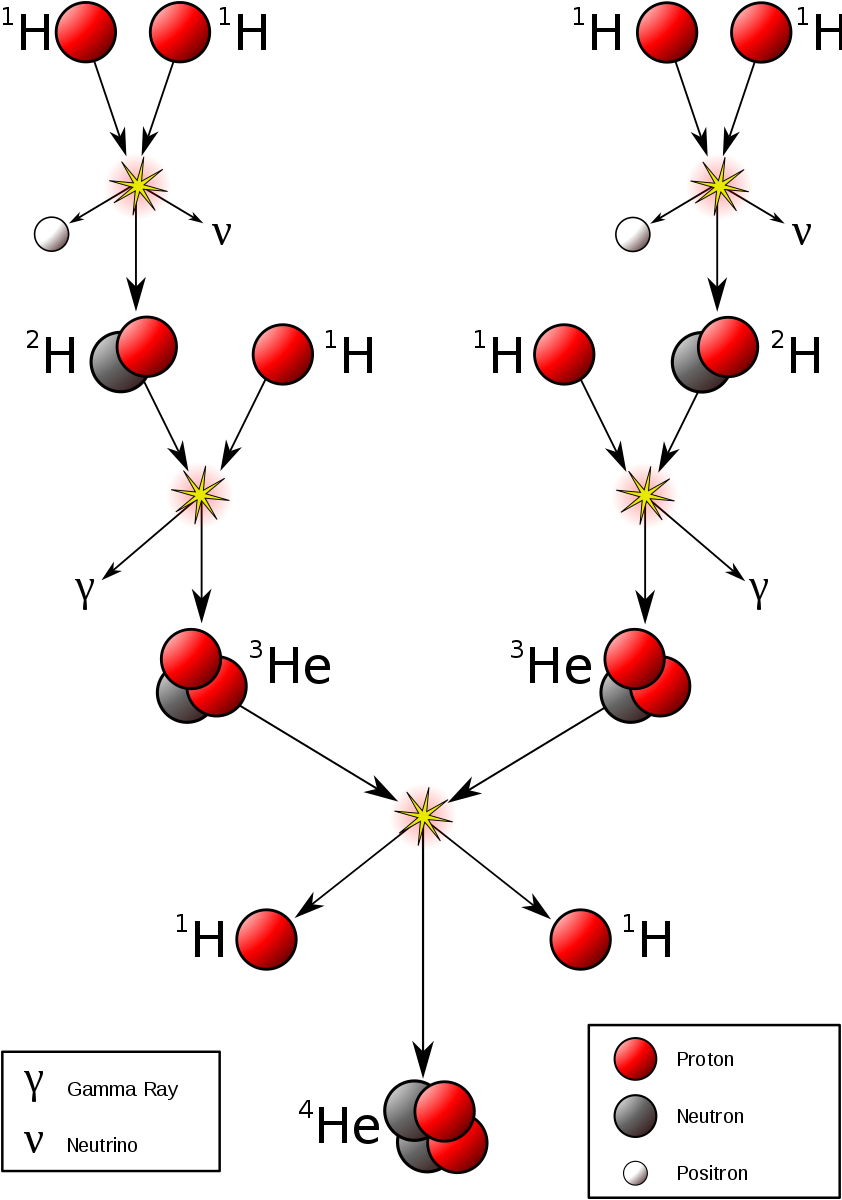
\includegraphics[height=0.8\textheight]{fusion-in-der-sonne}
\caption{Fusion in der Sonne}
\label{fig:fusion-in-der-sonne}
\end{figure}
\end{frame}

\begin{frame}{\subsecname}{\secname}
\pftn{https://de.wikipedia.org/wiki/Proton-Proton-Reaktion}
\begin{itemize}
\item \({\displaystyle \mathrm {{}^{1}H+{}^{1}H\to {}^{2}H+e^{+}+\nu _{e}+0{,}42\;MeV} }\)
\end{itemize}
\centering
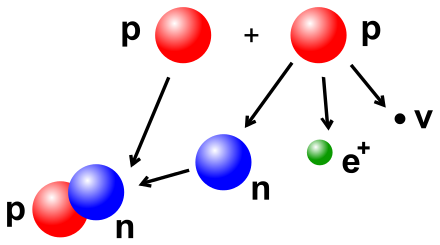
\includegraphics[height=0.4\textheight]{fids1}
\end{frame}

\begin{frame}{\subsecname}{\secname}
\pftn{https://de.wikipedia.org/wiki/Proton-Proton-Reaktion}
\begin{itemize}
\item \({\displaystyle \mathrm {{}^{2}H+{}^{1}H\to {}^{3}He+\gamma +5{,}493\;MeV} }\)
\end{itemize}
\centering
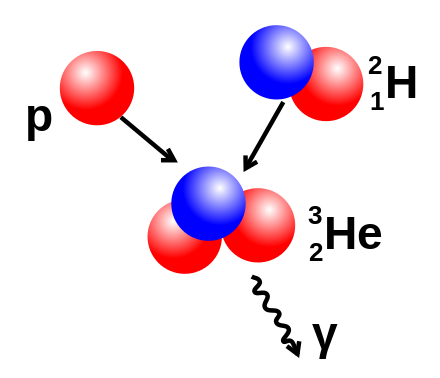
\includegraphics[height=0.5\textheight]{fids2}
\end{frame}

\begin{frame}[fragile]{\subsecname}{\secname}
\begin{figure}
\pftn{https://de.wikipedia.org/wiki/Datei:FusionintheSun.svg}
\centering
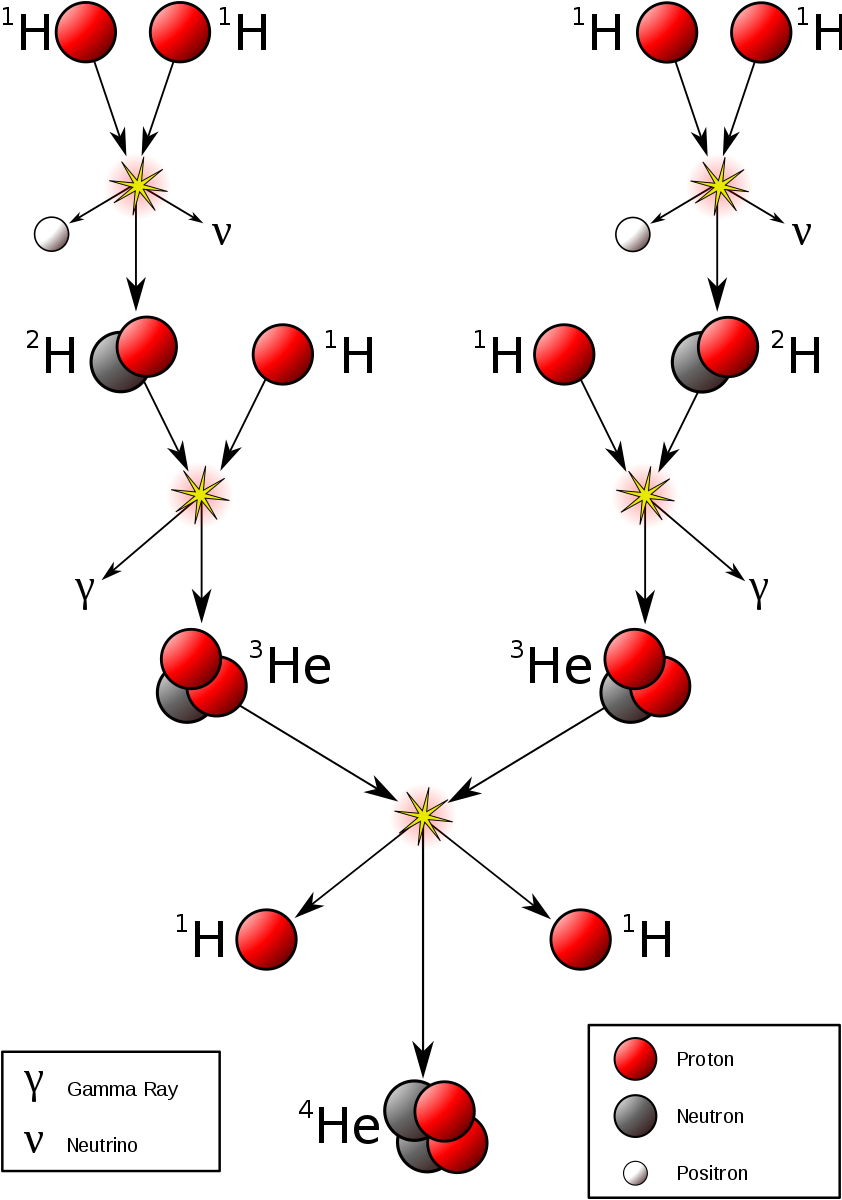
\includegraphics[height=0.8\textheight]{fusion-in-der-sonne}
\caption{Fusion in der Sonne}
\label{fig:fusion-in-der-sonne}
\end{figure}
\end{frame}

\begin{frame}{\subsecname}{\secname}
\pftn{https://de.wikipedia.org/wiki/Proton-Proton-Reaktion}
\begin{itemize}
\item Proton-Proton-I-Kette: 83,30 \%
\item \({\displaystyle \mathrm {{}^{3}He+{}^{3}He\to {}^{4}He+2\,{}^{1}H+12{,}86\;MeV} }\)
\end{itemize}
\centering
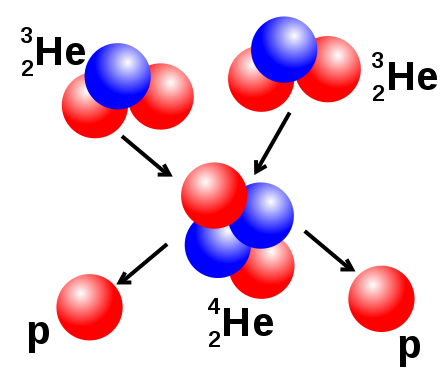
\includegraphics[height=0.5\textheight]{fids3}
\end{frame}

\begin{frame}{\subsecname}{\secname}
\pftn{https://de.wikipedia.org/wiki/Proton-Proton-Reaktion}
\begin{itemize}
\item Proton-Proton-I-Kette: 83,30 \%
\item Proton-Proton-II-Kette: 16,68 \%
\begin{itemize}
 \item 2x \({\displaystyle \mathrm {{}^{4}He}}\)
\end{itemize}
\item Proton-Proton-III-Kette: 0,02 \%
\begin{itemize}
	\item 2x \({\displaystyle \mathrm {{}^{4}He}}\)
\end{itemize}
\end{itemize}
\end{frame}


\subsection{Wasserstoffbombe}
\begin{frame}{\subsecname}{\secname}
\pftn{https://www.focus.de/7546710}
\LARGE Atombombe: \normalsize
\begin{itemize}
\item Sprengstoff verdichtet Spaltmaterial
\item => Kettenreaktion wird ausgelöst 
\end{itemize}
\pause
\LARGE Wasserstoffbombe: \normalsize
\begin{itemize}
\item Atombombe verdichtet Spaltmaterial
\item => Fusionsreaktionen beginnen
\end{itemize}
\end{frame}

\begin{frame}{\subsecname}{\secname}
\pftn{https://de.wikipedia.org/wiki/Datei:BombH\_explosion.svg}
\begin{figure}
\centering
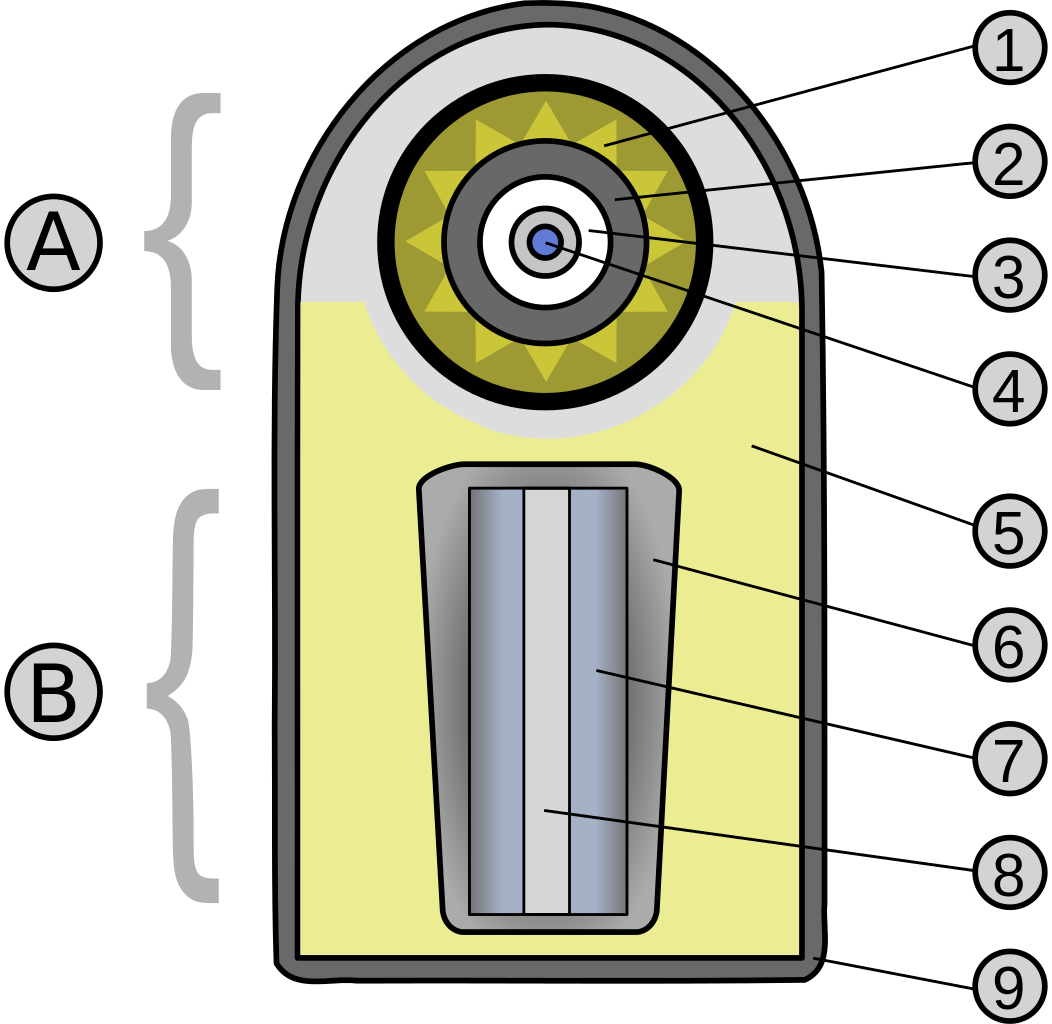
\includegraphics[height=0.8\textheight]{h-bomb}
\caption{Wasserstoffbombe}
\label{fig:h-bomb}
\end{figure}
\end{frame}

\begin{frame}{\subsecname}{\secname}
\pftn{https://de.wikipedia.org/wiki/Datei:BombH\_explosion.svg}
\begin{figure}
\centering
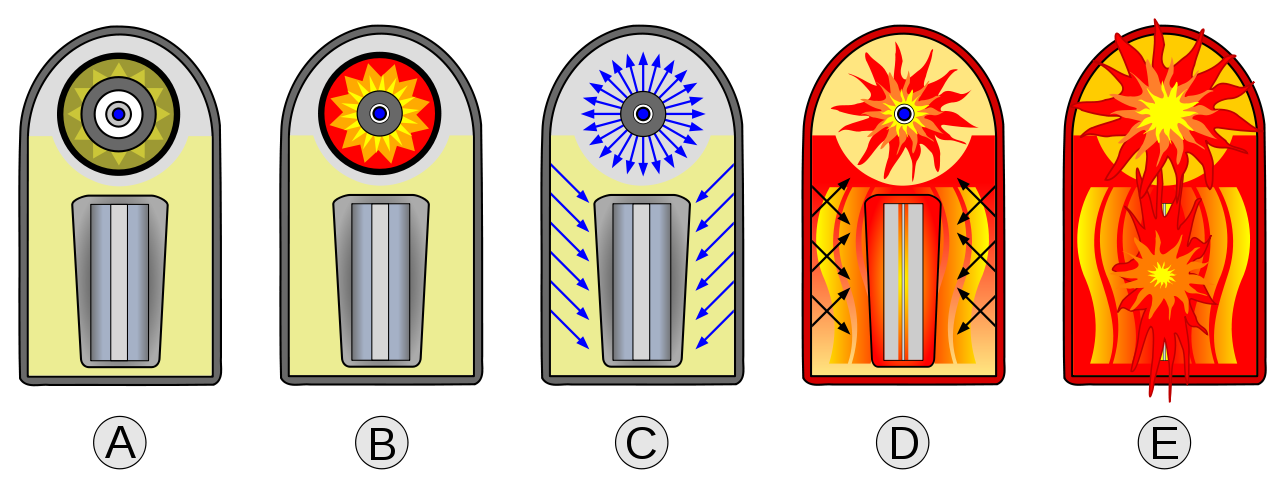
\includegraphics[width=\linewidth]{h-bomb-expl}
\caption{Explosion einer Wasserstoffbombe}
\label{fig:h-bomb-expl}
\end{figure}
\end{frame}


\section{Fusionsreaktor}
\subsection[Magnetische Fusion]{Magnetische Fusion (Tokamak / Stellerator)}
\begin{frame}{\subsecname}{\secname}

\end{frame}

\subsection{Trägheitsfusion}
\begin{frame}{\subsecname}{\secname}

\end{frame}

\subsection{Aufbau eines Reaktors}
\begin{frame}{\subsecname}{\secname}

\end{frame}

\subsection{Erbrütung von Tritium}
\begin{frame}{\subsecname}{\secname}

\end{frame}

\subsection{Sicherheit der Reaktoren}
\begin{frame}{\subsecname}{\secname}

\end{frame}



\begin{frame}
\titlepage
\end{frame}
\end{document}


%%  Energie aus Masse E=mc²
%% Geschichtlicher Überblick der Forschung
%% Unterwelchen Bedingungen funktioniert die Fusion (Hitze, Druck)
%% Fusion in der Sonne. In welchen Zonen und in welchen Lebenzzyklen finden welche Fusionsreaktionen statt.
%% Wasserstoffbombe: Erste Fusion auf der Erde.
%% Zwei Prinzipien der Fusionsreaktoren: magnetische Fusion (Tokamak / Stellarator), Trägheitsfusion
%% Aufbau eines Reaktors
%% Erbrütung von Tritium
%% Sicherheit von Fusionsreaktoren 
